\documentclass[a4paper]{article}
\usepackage[14pt]{extsizes}
\usepackage{setspace,amsmath}
\usepackage{savesym}
\savesymbol{iint}
\usepackage{txfonts}
\restoresymbol{TXF}{iint}
\usepackage[left=20mm, top=20mm, right=20mm, bottom=20mm]{geometry}
\setlength{\parindent}{12,5mm}
\linespread{1.15}
\usepackage[russian]{babel}
\usepackage[T2A]{fontenc} % кодировка
\usepackage{fontspec} 
\defaultfontfeatures{Ligatures={TeX}, Renderer=Basic} 
\setmainfont[Ligatures={TeX,Historic}]{Times New Roman}
\usepackage{graphicx}
\usepackage{lscape}
\usepackage{pdfpages}
\usepackage{hyperref}
\graphicspath{{pictures}}
\DeclareGraphicsExtensions{.pdf,.png,.jpg}
\begin{document}
\begin{titlepage}
\begin{center}
    \large{Министерство образования Республики Беларусь}\\
\large{Белорусский национальный технический университет}\\
\large{Факультет транспортных коммуникаций}\\
\large{Кафедра «Геодезия и аэрокосмические геотехнологии»}\\
\hfill \break
\hfill \break
\hfill \break
\hfill \break
\hfill \break
\hfill \break
\textbf{\LARGE{Отчет}\\
\Large{по учебно-геодезической практике\\
(Высшая геодезия)\\}}
\hfill \break
\hfill \break
\hfill \break
\end{center}
\begin{flushright}
  \large{Выполнил: Бригада № 3\\
 Смоуж Т. А.\\
 Лаппо Я. В.\\
 Гайдук А. С.\\
 Малец Е. Д.\\
 Проверил: Будо А. Ю.\\}
\end{flushright}
\begin{center}
\hfill \break
\large{Минск, 2021\\}
\end{center}
\end{titlepage}
\setcounter{page}{3}
% Оглавление будет в виде пдф подшитого в латех
\begin{center}
    \large{\textbf{ПОЛИГОНОМЕТРИЯ 4 КЛАССА 1 И 2 РАЗРЯДОВ}}
\end{center}
\large{
\par Полигонометрические сети 4 класса, 1 и 2 разрядов создаются в виде отдельных ходов или различных систем ходов.
\par Отдельный ход полигонометрии должен опираться на 2 исходных пункта. На исходных пунктах необходимо измерять примычные углы.
\par В исключительных случаях при отсутствии между исходные пунктами видимости с земли допускается:
\par - проложение хода полигонометрии, опирающегося на 2 исходных пункта, без угловой привязки на одном из них. Для контроля угловых измерений используются дирекционные углы на ориентирные пункты государственной геодезической сети или дирекционные углы примычных сторон;
\par- проложение замкнутого хода полигонометрии 1, 2 разрядов опирающегося на один исходный пункт, при условии передачи или измерения с точек хода двух дирекционных углов на две смежные стороны по возможности в середине хода;
\par- координатная привязка к пунктам геодезической сети. При этом для контроля угловых измерений в целях обнаружения грубых ошибок измерений используются дирекционные углы на ориентирные пункты или азимуты, полученные из астрономических или гиротеодолитных измерений.
\par Проложение висячих ходов не допускается.
\par При построении полигонометрических сетей 4 класса, 1 и 2 разрядов необходимо соблюдать следующие требования, приведенные, таблице 1.\\
\\
\\
\\
Таблица 1 $-$ Требования к полигонометрии 4 класса.\\
\begin{tabular}{|l|c|c|c|}
\hline
Показатели & 4 класс & 1 разряд & 2 разряд \\
\hline
Предельная длина хода: & & & \\
отдельного & 15 км & 5 км & 3 км \\
между исходной и узловой точкой & 10 км & 3 км & 2 км\\
между узловыми точками& 7 км & 2 км & 1,5 км \\
\hline
Предельный параметр полигона & 30 км & 15 км & 9 км \\
\hline
Длины сторон хода: & & & \\
наибольшая & 2,00 км & 0,80 км & 0,35 км \\
наименьшая & 0,25 км & 0,12 км & 0,08 км \\
средняя расчетная & 0,50 км & 0,30 км  & 0,20 км \\
\hline
Число сторон в ходе, не более & 15& 15& 15\\
\hline
Относительная погрешность & 1:25000 & 1:10000 & 1:5000\\
\hline
СКП измерения угла не более & 3" & 5" & 10"\\
\hline
Угловая невязка хода, не более & $5\sqrt{n}$ & $10\sqrt{n}$ & $20\sqrt{n}$ \\
\hline
\end{tabular}
\hfill \break
\par Расстояние между пунктами параллельных полигонометрических ходов данного класса, по длине близких к предельным, должно быть не менее:
\par - в полигонометрии 4 класса - 2,5 км;
\par - 1 разряда - 1,5 км. 
\par С целью обеспечения большей жесткости сети следует стремиться к сокращению многоступенчатости сети, ограничиваясь развитием полигонометрии 4 класса и 1 разряда.
\par Измерение углов на пунктах полигонометрии производится способом измерения отдельного угла или способом круговых приемов, как правило, по трехштативной системе. При этом для приборов должны соблюдаться допуски, приведенные в таблице 2.
\par Так как измерения производились теодолитом с точность 2", то в таблице 2 приведены допуски для приборов соответствующей точности.\\
Таблица 2 $-$ Допуски при измерении горизонтальных углов.\\
\begin{tabular}{|c|c|}
\hline
Основные элементы угловых измерений & Допуски для 2" \\

\hline
Расхождения в полуприёмах & 8" \\
\hline
Расхождения в приёмах & 8" \\
\hline
Колебание значения 2С в приёмах & 12" \\
\hline
Колебание между повторными &  \\
наблюдениями начального направления & 8" \\
в начале и конце полуприёма &  \\
\hline
Колебание направлений в отдельных приёмах & 8" \\
\hline
\end{tabular}
\\
\par Теодолит и визирные цели должны устанавливаться над центрами с точностью 1 мм с помощью оптического центрира.
\par Линии в полигонометрии 4 класса, 1 и 2 разрядов измеряются светодальномерами, радиодальномерами. 
\par В отдельных случаях - базисными приборами, тахеометрами и другими приборами и методами, обеспечивающими точность, соответствующую классу или разряда полигонометрии.
\par Приборы и оборудование, фиксирующие концы линии, должны устанавливаться над центрами с точностью 1 мм.
\begin{newpage}
\begin{center}
    \large{\textbf{НИВЕЛИРОВАНИЕ III КЛАССА}}
\end{center}
 \par Способ нивелирования III класса зависит от применяемых нивелиров. Предпочтение отдают нивелирам с компенсатором. Нивелиры и рейки исследуют и поверяют с целью установления их пригодности для нивелирования III класса, приведения в рабочее состояние и определения постоянных.
 \par Нивелирование III класса производят в прямом и обратном направлениях.
  \par Порядок работы на станции при использовании цифрового нивелира и штриховой рейки:
  \par 1. Прибор устанавливается на равноудаленное расстояние между двумя рейками и приводится в рабочее положение.
  \par 2. Наводятся на заднюю рейку, берут отсчет и записывают его в журнал нивелирования. \par 3. Наводятся на переднюю рейку, берут отсчет и записывают его в журнал нивелирования.
  \par 4. Меняют высоту инструмента.
  \par 5. Наводятся на переднюю рейку, берут отсчет и записывают его в журнал нивелирования.
  \par 6. Наводятся на заднюю рейку, берут отсчет и записывают его в журнал нивелирования.
  \par 7. Выполняют постраничный контроль. 
 \par Нивелирование выполняют участками в 20-30 км. Переход от нивелирования в прямом направлении к нивелированию в обратном направлении делают только на постоянных знаках. При этом рейки меняют местами. 
\par Нормальная длина луча визирования - 75 м. При отсутствии колебаний изображения реек и увеличения трубы не менее 35х длину луча разрешается увеличивать до 100 м. Неравенство расстояний на станции допускают не более 2 м, а их накопление по секции - не более 5 м.
\par Высота луча визирования над подстилающей поверхностью должна быть не менее 0,3 м. \par Нивелирование выполняют при хорошей видимости, отчетливых и спокойных изображениях реек. В солнечные дни не следует нивелировать в периоды, близкие к восходу и заходу солнца.
\par При работе на станции нивелир с уровнем защищают от солнечных лучей зонтом.
\par Рейки устанавливают по уровню на костыли или башмаки. В местах установки башмаков предварительно снимают дерн. Для удобства рекомендуется пользоваться не менее чем тремя костылями или башмаками. На участках с рыхлым или заболоченным грунтом рейки устанавливают на забитые деревянные колья с вбитыми в их торцы гвоздями с полусферическими головками. Длина и диаметр кольев должны быть такими, чтобы обеспечивалась их устойчивость.
\par После выполнения нивелирования по секции сравнивают между собой значения превышения, полученные из прямого и обратного ходов; расхождение между этими значениями не должно превышать 10 мм . 
\par Если расхождение получилось больше допустимого, то нивелирование по секции повторяют в одном из направлений. Явно неудовлетворительное значение превышения исключают. Оставшиеся два значения принимают в обработку, если они не расходятся между собой больше чем на 10 мм и получены из нивелирования в противоположных направлениях.
\end{newpage}
\begin{newpage}
\begin{center}
    \large{\textbf{СПУТНИКОВЫЕ ИЗМЕРЕНИЯ}}
\end{center}
\par В настоящее время всё большую популярность приобретают методы определения координат и высот с применением спутниковой геодезической аппаратуры (в дальнейшем — СГА).
\par Данные методы по сравнению с традиционной, «наземной» технологией, имеют неоспоримые преимущества, которые проявляются в повышении производительности труда, снижении издержек производства инженерно-геодезических работ, и как результат — повышения качества продукции, снижение конечной стоимости этапов строительства зданий и сооружений, достижении конкурентоспособности предприятия.
\par Принцип спутникового метода измерения координат заключается в определении расстояния от приемника до спутника и последующей корректировки полученных данных с учетом поправок. Сегодня все работы проводятся в двух группах режимов, в статических и кинематических.
\par \textit{Статическая съемка} – это классический вид съемки, хорошо приспособленный для любой длины базовой линии (короткой, средней, длинной). Один приемник (базовый) находится на точке с известными координатами, другой устанавливают на точку, координаты которой необходимо определить, и производят одновременную запись измерений во внутреннюю память для их последующей обработки на компьютере и вычисления координат. Весь процесс измерений полностью автоматизирован. Время наблюдения зависит от длины базовой линии (расстояния от базового до подвижного приемника), количества видимых спутников и т.д. Как правило, одночастотные приемники используются на базовых линиях, длина которых не превышает 15 км. Для базовых линий длиннее 15 км следует использовать двухчастотные приемники.
\par Методика выполнения измерений в режиме «Статика»
\par - Прогнозирование (планирование измерений);
\par - Полевые работы;
\par - Предобработка;
\par - Уравнивание и оценка точности результатов измерений.
\begin{center}
    \large {\textbf{Прогнозирование (планирование измерений)}}
\end{center}
\par Оно выполняется основе предварительной полевой и камеральной подготовки материалов.
\par Полевая подготовка включает в себя:
\par - рекогносцировку;
\par - обследование исходных пунктов;
\par - закладку определяемых пунктов будущей спутниковой геодезической сети.
\par Камеральная подготовка:
\par - сбор и анализ исходных данных;
\par - изученности района работ, подготовка оборудования;
\par - выбор методов и проектирование геодезической сети;
\par - прогнозирование полевых наблюдений. 
\begin{center}
    \large {\textbf{Полевые работы}}
\end{center}
\par Измерения в режиме «Статика» подразумевают выполнение длительных наблюдений на пунктах сети. Наблюдения заключаются в одновременной работе двух и более приёмников СГА для определения векторов геодезической сети. Наблюдения выполняются согласно программе работ, при необходимости корректируя действия в зависимости от внешних условий.
\par Важно, чтобы приемники были проверены и полностью заряжены, для того что бы обеспечить непрерывность сеансов и работу в течение запланированного времени.
\begin{center}
    \large {\textbf{Предобработка}}
\end{center}
\par Измерения, полученные при выполнении полевых работ, загружаются с приёмников, импортируются в новый или ранее созданный проект программного комплекса.
\par Далее выполняется предварительная обработка с оценкой точности полученных параметров векторов, в результате которой принимается решение о принятии или исключении их в дальнейшей работе. Методика предварительной обработки и принятие решения о пригодности зависит от используемых программных комплексов. Наши измерения обрабатывались в программном продукте КРЕДО GNSS.
\begin{center}
    \large {\textbf{Уравнивание и оценка точности результатов измерений}}
\end{center}
\par После предобработки выполняется уравнивание результатов измерений в два этапа. На первом уравнивается вся сеть без фиксирования координат опорных пунктов. Особенность этапа заключается в отсутствии влияния ошибок координат исходных пунктов.
\par На втором этапе производится поочерёдная фиксация координат опорных пунктов с одновременным выполнением анализа о пригодности каждого пункта для выполнения уравнивания сети. В результате возможно принятие решений об исключении или необходимости добавления других опорных пунктов.
\par В результате уравнивания создаётся подробный отчёт, в котором проводится оценка качества выполненной работы, каталог уравненных координат и высот с оценкой точности каждого определяемого пункта. Пример такого отчёта:
\end{newpage}
}
\begin{titlepage}
\begin{flushright}
  \large{\textbf{ПРИЛОЖЕНИЕ А. Поверки электронного теодолита DT-2A}}
\end{flushright}
\begin{center}
\large{Белорусский национальный технический университет}\\
\large{Факультет транспортных коммуникаций}\\
\large{Кафедра «Геодезия и аэрокосмические геотехнологии»}\\
\hfill \break
\hfill \break
\hfill \break
\hfill \break
\hfill \break
\hfill \break
\large{Отчет\\
 о выполнении поверок электронного теодолита DT-2A }\\
\hfill \break
\hfill \break
\hfill \break
\hfill \break

\end{center}
\begin{flushright}
  \large{Выполнил: Бригада № 3\\
	Лаппо Я.В.\\
	Смоуж Т. А.\\
	Малец Е.Д.\\
	Гайдук А.С.\\
	\hfill \break
	Проверил: ст. преподаватель\\
	Будо А. Ю.\\}
\end{flushright}
\begin{center}
\hfill \break
\hfill \break
\large{Минск, 2021\\}
\end{center}
\end{titlepage}
\setcounter{page}{14}
\large{\textbf{1. Поверка цилиндрического уровня}
\par \textbf{Главное условие:} Ось цилиндрического уровня должна быть перпендикулярна вертикальной оси инструмента.
\par \textbf{Выполнение поверки:} Установите инструмент так, чтобы ось цилиндрического уровня была параллельна
двум установочным винтам. С помощью этих винтов загоните пузырь уровня в центр колбы уровня.
\par Поверните инструмент на 180˚ вертикальной оси и проверьте движение пузыря цилиндрического уровня. Если пузырь переместился, следует выполнить юстировку.
\par \textbf{Результат поверки:} Пузырек уровня отклонился на 1/2 деления от нуль-пункта.
\par\textbf{Вывод:} Поверка выполняется.
\par \textbf{Юстировка:} Отрегулируйте положение пузырька уровня с помощью шпильки из набора
аксессуаров к инструменту, чтобы он переместился к центру колбы на половину своего отклонения.
\par Откорректируйте оставшуюся половину отклонения с помощью установочных
винтов.
\par Поверните инструмент на 180˚ вертикальной оси и проверьте движение пузыря цилиндрического уровня. Если пузырь переместился, следует повторить регулировку.
\par\textbf{2. Поверка круглого уровня}
\par \textbf{Главное условие:} Ось круглого уровня должна быть параллельна оси вращения инструмента.
\par \textbf{Выполнение поверки:} До начала данной поверки должна быть выполнена юстировка цилиндрического уровня (если в этом есть необходимость). Если пузырёк круглого уровня находится в нуль-пункте после приведения в центр пузырька цилиндрического уровня, то дальнейшая юстировка не требуется. В противном случае необходима юстировка. 
\par \textbf{Результат поверки:} Пузырёк круглого уровня находится в нуль-пункте после приведения в центр пузырька цилиндрического уровня.
\par\textbf{Вывод:} Поверка выполняется.
\par \textbf{Юстировка:} Действуя юстировочной шпилькой, повернуть юстировочные винты, пока пузырёк круглого уровня не переместится в центр. Во избежание разрыва, нельзя перетягивать юстировочные винты.
\par\textbf{3. Поверка сетки нитей телескопа}
\par \textbf{Главное условие:} Вертикальные нити сетки нитей телескопа должны быть перпендикулярны горизонтальной оси инструмента.
\par \textbf{Выполнение поверки:} Тщательно отгоризонтируйте инструмент на треггере.
\par Наведите сетку нитей на хорошо видимую точку А с дистанции не менее 50 м.
\par Качните телескоп по вертикали и проверьте скользит ли точка А вдоль всей
вертикальной нити.
\par Если точка А скользит вдоль всей вертикальной нити, то вертикальные нити сетки
нитей телескопа перпендикулярны горизонтальной оси инструмента. Юстировка в этом случае не требуется.
\par Если точка А при качении оптической трубы вдоль вертикали отклоняется от
вертикальной нити сетки нитей, то в этом случае юстировка требуется.
\par \textbf{Результат поверки:} Точка А скользит вдоль всей вертикальной нити.
\par\textbf{Вывод:} Поверка выполняется.
\par \textbf{Юстировка:} Отвинтите крышку покрывающую 4 регулировочных винта сетки нитей поворачивая
крышку против часовой стрелки.
\par Ослабте эти винты отверткой из набора аксессуаров, считая при этом число оборотов
отвёртки. Совместите вертикальную нить сетки нитей с точкой А и затяните
регулировочные винты тем же количеством оборотов отвёртки.
\par Проведите проверку  до тех пор пока точка А не будет скользить по всей длине вертикальной нити сетки нити.

\par\textbf{4. Коллимация инструмента}
\par \textbf{Главное условие:} Визирная ось телескопа должна быть перпендикулярна горизонтальной оси инструмента.
\par \textbf{Выполнение поверки:} Установите инструмент между точками А и В в пределах их прямой видимости на равном расстоянии 50 – 60м от каждой из них.
\par Тщательно отгоризонтируйте инструмент на триггере по цилиндрическому уровню.
\par Наведитесь на А.
\par Ослабьте затяжной винт вертикальной наводки и поверните трубу на 180˚ вокруг горизонтальной оси инструмента т.о. чтобы труба показывала в
противоположную сторону
\par Наведитесь на точку В и закрепите затяжной винт вертикальной наводки.
\par Ослабте затяжной винт горизонтальной наводки и поверните трубу на 180˚ вокруг вертикальной оси инструмента т.о. чтобы труба показывала в
противоположную сторону. Наведитесь на точку А и закрепите затяжной винт
горизонтальной наводки.
\par Ослабьте затяжной винт вертикальной наводки и поверните трубу на 180˚
вокруг горизонтальной оси инструмента. Перекрестие сетки нитей телескопа (точка С)
должно совпасть с точкой В.
\par Если точка С не совпадает с точкой В то требуется регулировка состоящая из
следующих процедур.
%\begin{center}
    %\fbox {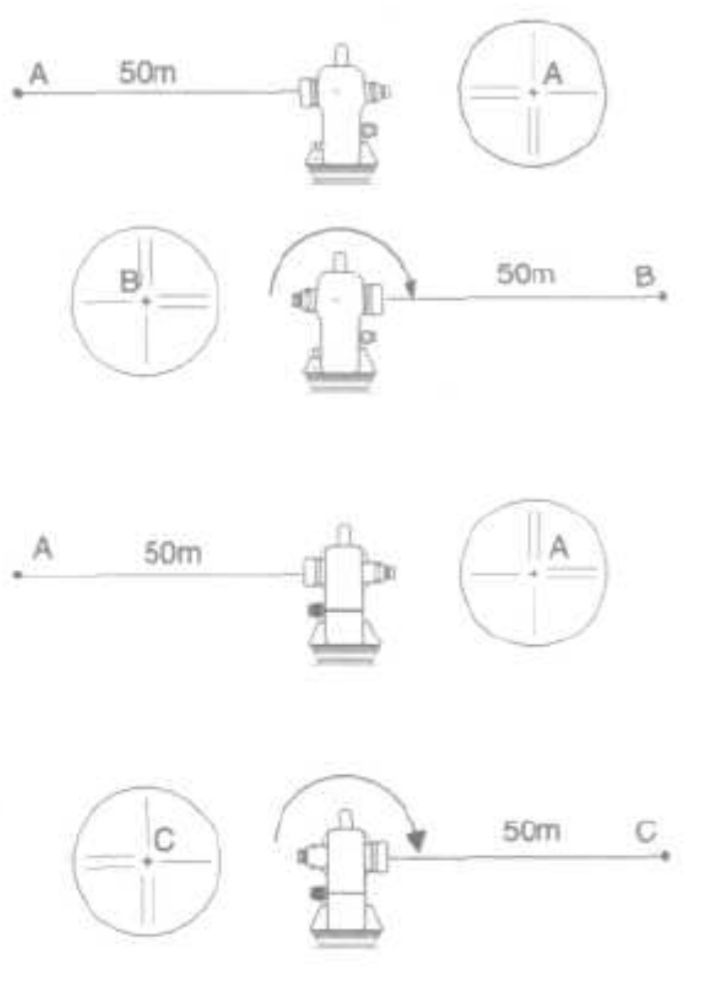
\includegraphics[scale=0.45]{photo1625172362.jpeg} }\\
   % Рисунок 1 $-$ \textit{«Коллимация инструмента»}  
%\end{center}
\par \textbf{Результат поверки:} Точки совпадают.
\par\textbf{Вывод:} Поверка выполняется.
\par \textbf{Юстировка:} Отвинтите крышку покрывающую 4 регулировочные винты сетки нитей. Регулировочных винта сетки нитей поворачивая крышку против часовой стрелки
\par Определите точку D между В и С т.о. чтобы расстояние CD равнялось ¼ расстояния ВС. (несовпадение ВС в 4 раза больше реальной ошибки за коллимацию из-за того что телескоп при проверке поворачивался 2 раза.
\par Поворачивая регулировочные воротки в верхней, нижней, левой и правой части
окуляра передвиньте вертикальную нить сетки нитей т.о. чтобы она совпадала с точкой
D. По окончании регулировки повторите процедуру проверки. 
\par Если точки В и С совпадают, то дальнейшей регулировки не требуется. В противном случае повторите
регулировку.
\par\textbf{5. Поверка лазерного отвеса.}
\par \textbf{Главное условие:} Вертикальная ось теодолита должна находиться над
точкой центрирования когда лазерный визир будет попадать на точку центрирования.
\par \textbf{Выполнение поверки:} Установите инструмент на штатив на высоту около 1.5м и отгоризонтируйте его. Включите лазерный отвес и заметьте первоначальное расположение лазерного визира на
земле.
\par Поверните инструмент на 180˚ вокруг вертикальной оси и проверьте точку на
земле. Если первоначальная точка центрирования остаётся в пределах 1мм от
первоначального положения визира регулировки не требуется. В противном случае
требуется регулировка состоящая из следующих процедур.
\par \textbf{Результат поверки:} Точка центрирования остаётся в пределах 1мм от
первоначального положения визира.
\par\textbf{Вывод:} Поверка выполняется.
\par \textbf{Юстировка:} Отвинтите крышку регулировочной части окуляра отвеса. Под ней находятся 4
регулировочных винта воротков. Отрегулируйте положение воротков окуляра с
помощью шпильки из набора аксессуаров т. о. чтобы передвинуть
первоначальную точку центрирования к лазерному визиру на ½ величины её
отклонения от визира.
\par Поверните инструмент на 180˚ вокруг вертикальной оси и проверьте точку на
земле. Если первоначальная точка центрирования остаётся менее 1мм от первоначального
положения визира регулировки не требуется. В противном случае требуется повторение
регулировки.
}
\begin{titlepage}
\begin{flushright}
  \large{\textbf{ПРИЛОЖЕНИЕ Б. Поверки цифрового нивелира DL-202}}
\end{flushright}
\begin{center}
\large{Белорусский национальный технический университет}\\
\large{Факультет транспортных коммуникаций}\\
\large{Кафедра «Геодезия и аэрокосмические геотехнологии»}\\
\hfill \break
\hfill \break
\hfill \break
\hfill \break
\hfill \break
\hfill \break
\hfill \break
\hfill \break
\large{Поверки электронного нивелира \textit{DL$-$ 202}\\}
\hfill \break
\hfill \break
\hfill \break
\hfill \break
\hfill \break
\hfill \break
\end{center}
\begin{flushright}
  \large{Выполнил: Бригада № 3 \\
	Лаппо Я. В\\
	Смоуж Т. А.\\
	Гайдук А. С.\\
	Малец Е. Д.\\
	}
\end{flushright}
\begin{center}
\hfill \break
\hfill \break
\large{Минск, 2021\\}
\end{center}
\end{titlepage}
\setcounter{page}{21}
\large{
\par\textbf{1. Поверка круглого уровня}
\par \textbf{Главное условие:} Ось круглого уровня должна быть параллельна оси вращения инструмента.
\par \textbf{Выполнение поверки:} Подъемными винтами подставки выводят в центр окружности пузырек установочного круглого уровня.
\par Поворачивают зрительную трубу вокруг оси вращения инструмента на 180°.
\par Если пузырек круглого уровня после поворота трубы остался в центре, то условие поверки выполнено, в противном случае необходимо произвести юстировку круглого уровня.
\par \textbf{Результат поверки:} Юстировка не требуется.
\par \textbf{Юстировка:} выполняется следующим образом:
\par - исправительными винтами круглого уровня перемещают пузырек к центру на половину его отклонения;
\par - подъемными винтами подставки устраняют вторую половину отклонения, т.е. выводят пузырек уровня точно на центр.
Для контроля поверку повторяют.
\par\textbf{2. Поверка сетки нитей}
\par \textbf{Главное условие:} Горизонтальная нить сетки должна быть перпендикулярна вертикальной оси вращения инструмента.
\par \textbf{Выполнение поверки:} Устанавливают и приводят в рабочее положение нивелир, а на расстоянии 30-40 мм от него устанавливают рейку.
\par Наводят зрительную трубу нивелира на рейку так, чтобы ее изображение оказалось на краю поля зрения, закрепляют трубу и берут отсчет по рейке.
\par Наводящим винтом перемещают трубу в горизонтальной плоскости до так пор, пока изображение рейки окажется на другом краю поля зрения, и берут по рейке еще один отсчет.
\par Если отсчеты равны, то условие поверки выполнено, в противном случае необходимо произвести юстировку сетки нитей.
\par \textbf{Результат поверки:} Юстировка не требуется.
\par \textbf{Юстировка:} выполняется следующим образом:
\par - отвинчивают колпачок окулярной части трубы;
\par - ослабляют крепежные винты оправы сетки нитей;
\par - поворачивают оправу сетки нитей так, чтобы ее горизонтальная нить оказалась на отсчете;
\par - зажимают крепежные винты оправы сетки и завинчивают колпачок обратно на окулярную часть трубы.
\par\textbf{3. Поверка главного условия}
\par \textbf{Главное условие:} Визирная ось зрительной трубы должна быть перпендикулярна вертикальной оси прибора.
\par \textbf{Выполнение поверки:} Две нивелирные рейки устанавливаются в створе на расстояние 50 м друг от друга (A и B). Следующим шагом необходимо устанавливают нивелир от рейки B на расстояние, примерно одна треть от общего, и приводят прибор в рабочее положение. 
\par Далее выполняют следующую последовательность действий: \textbf{Menu → Measure → Adjust}. Четко наводятся на рейку и нажимают \textbf{Meas}. В результате, прибор самостоятельно берет отсчет по рейке А. После чего нажимают \textbf{Ent} и наводятся на рейку В, далее еще раз нажимают \textbf{Meas}. В результате, прибор самостоятельно берет отсчет по рейке В.
\par Следующим шагом, нивелир устанавливают от рейки А на расстояние, примерно одна треть от общего, и приводят прибор в рабочее положение.После нажатия на \textbf{Ent} и наводятся на рейку В, далее нажимают \textbf{Meas}. В результате, прибор самостоятельно берет отсчет по рейке В. Нажимают \textbf{Ent} и наводятся на рейку А, далее нажимают \textbf{Meas}, в результате прибор самостоятельна берет отсчет по рейке А.
\par После выполнения всего вышеперечисленного прибор самостоятельно рассчитывает величины отклонений, которые сравниваются с допусками и на основе сравнения делается вывод о необходимости выполнения юстировки.
\par \textbf{Допуск:} При расстоянии 50 м, величина угла \textit{i} не должна превышать $10^{''}$, а величина отклонения \textit{x} не должна превышать 3 мм. 
\par \textbf{Результат поверки:} Юстировка не требуется.
}
\begin{newpage}
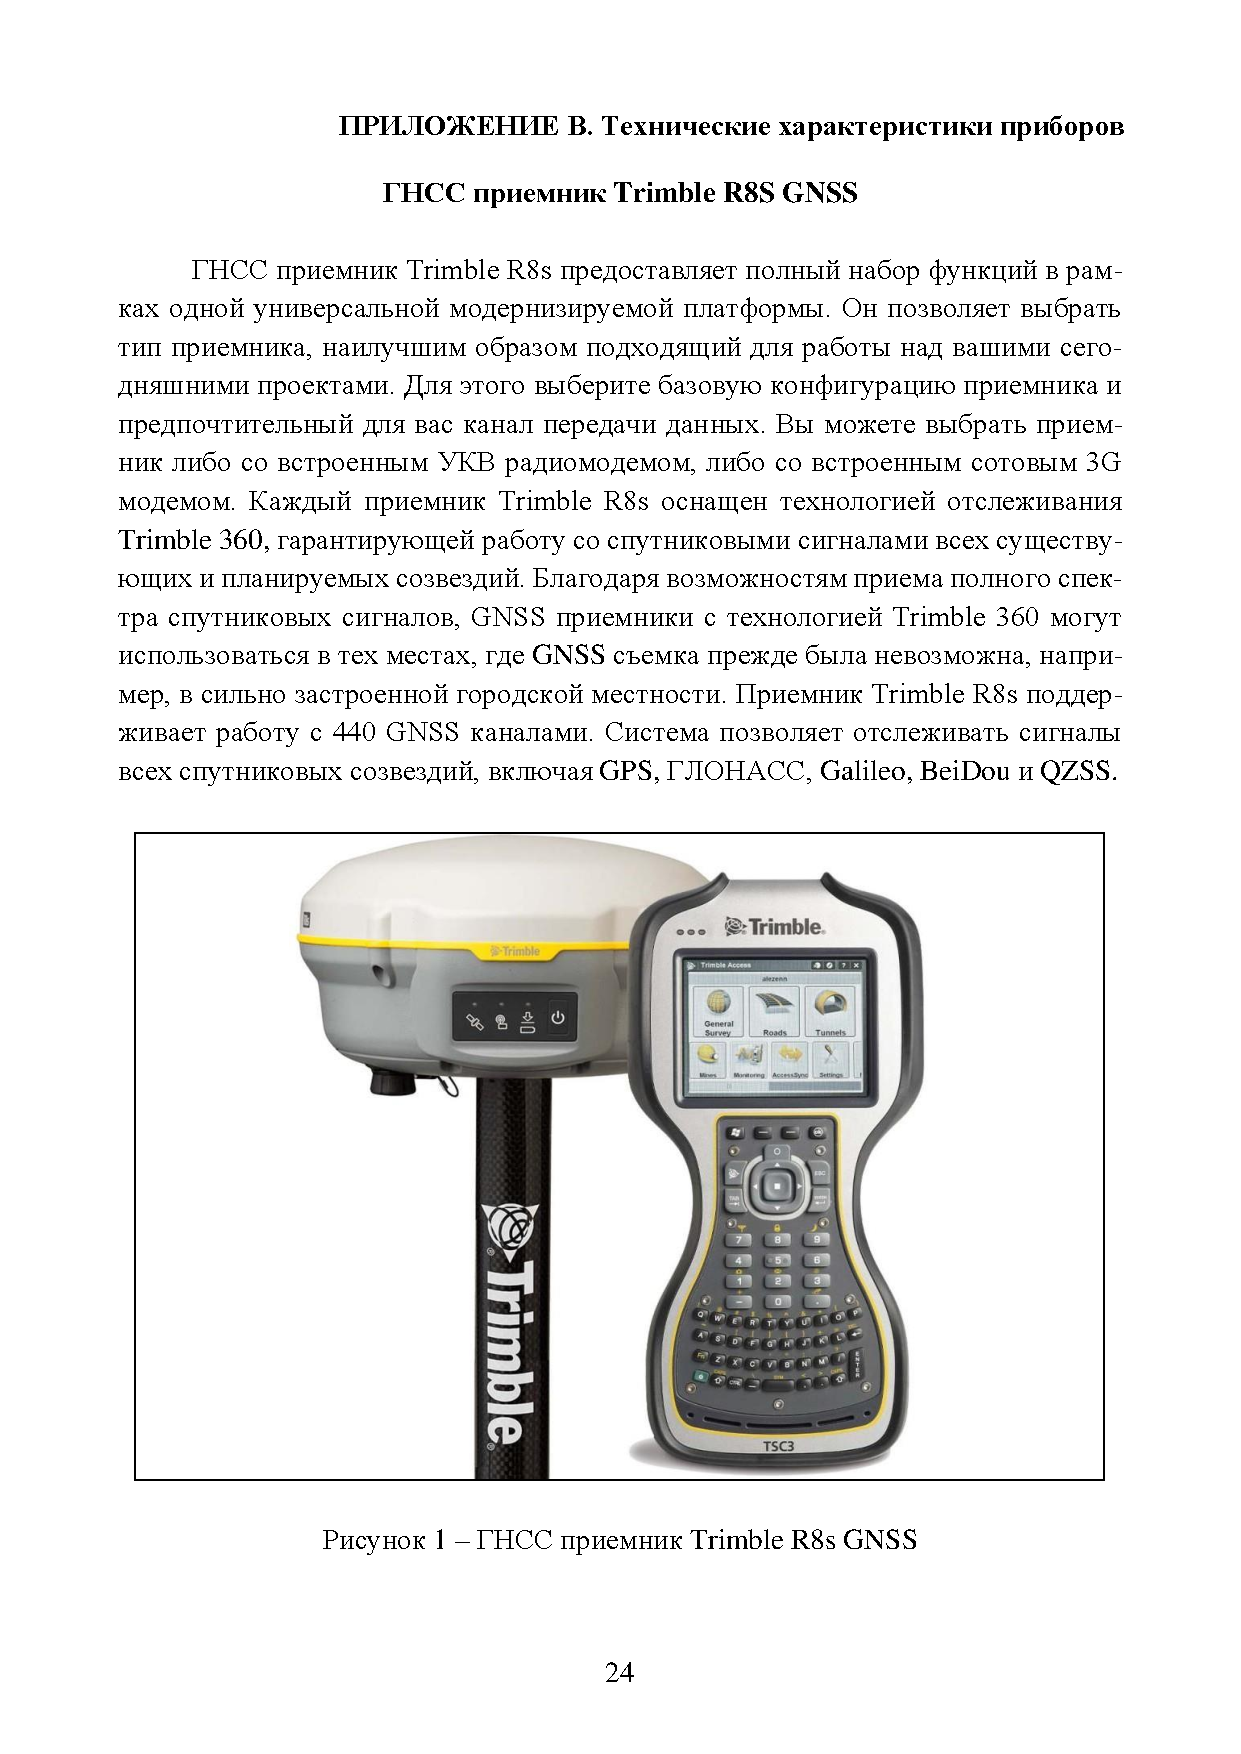
\includepdf[pages= - ]{Технические характеристики пиборов.pdf}
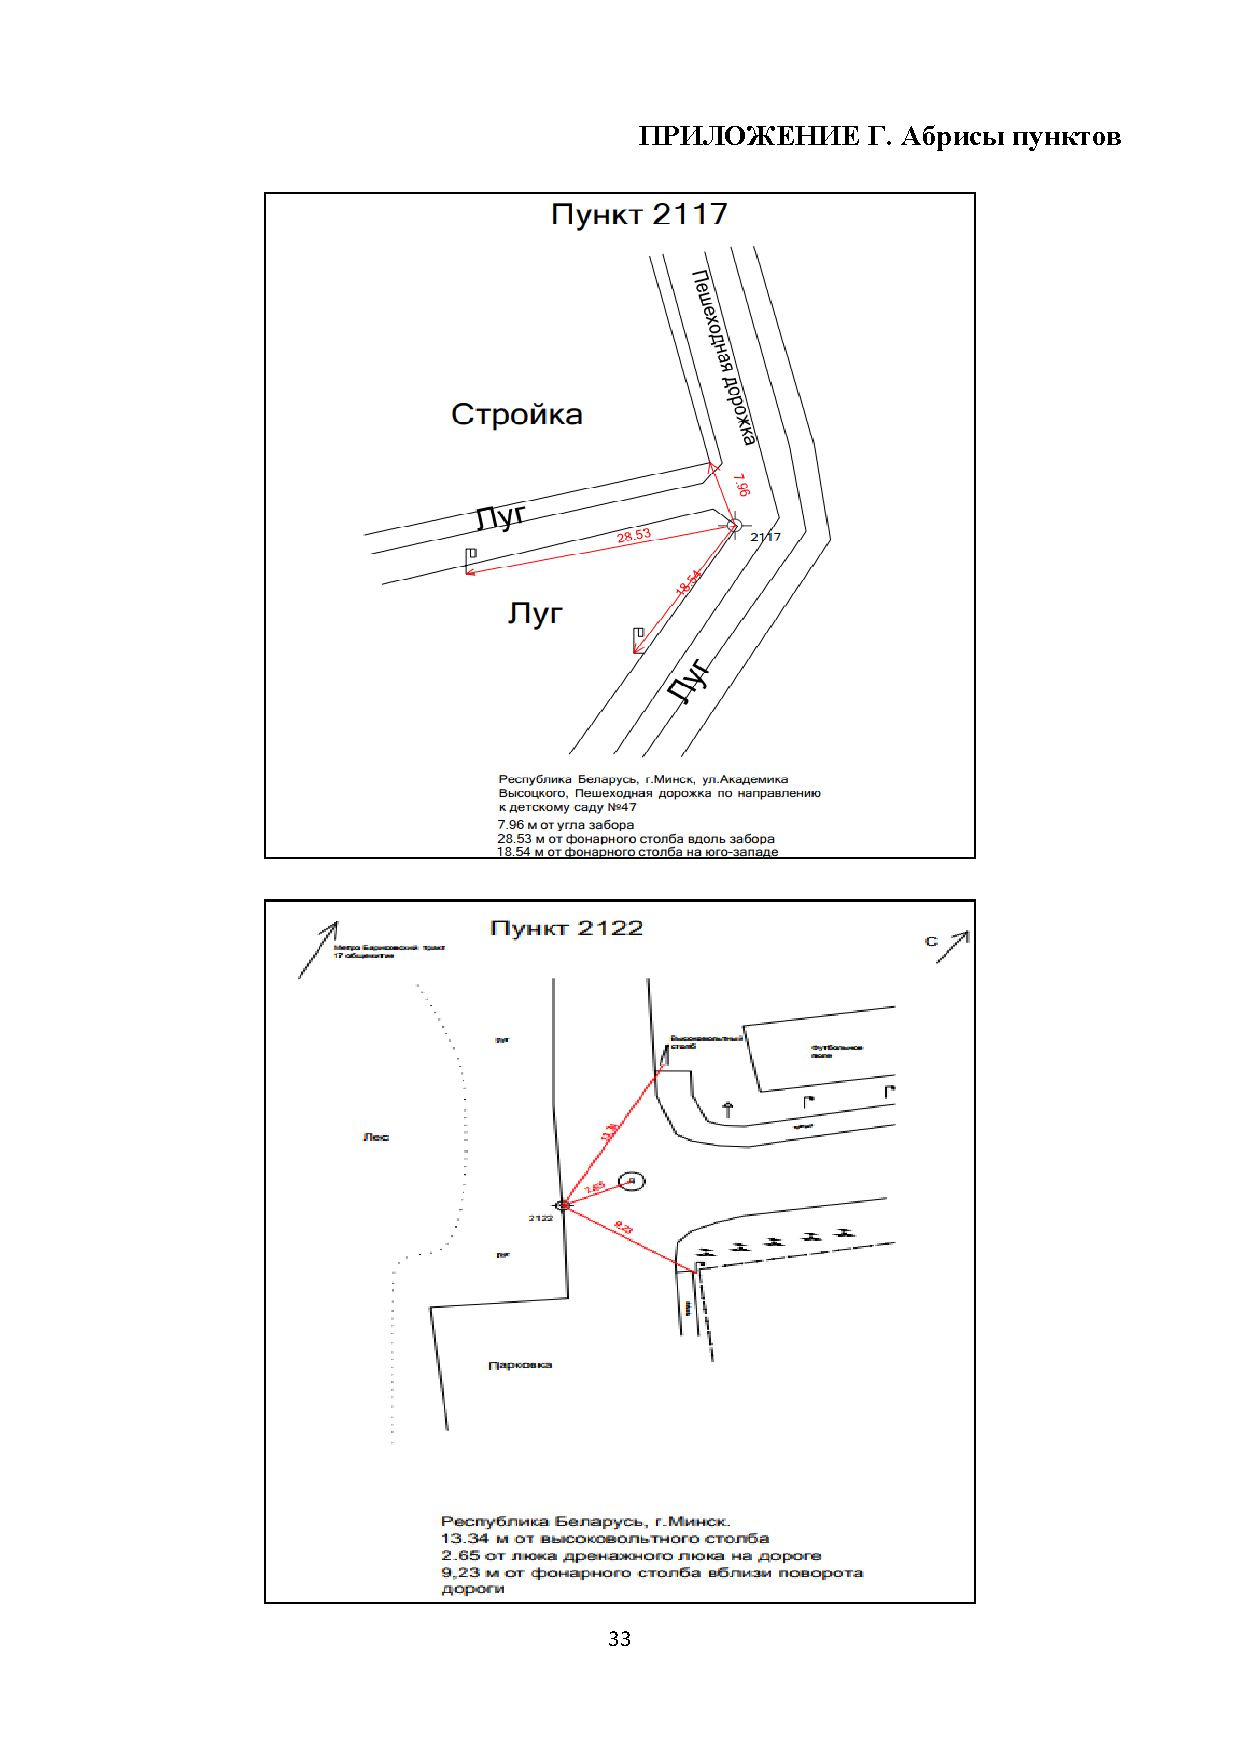
\includepdf[pages= - ]{2117 - 2131.pdf}
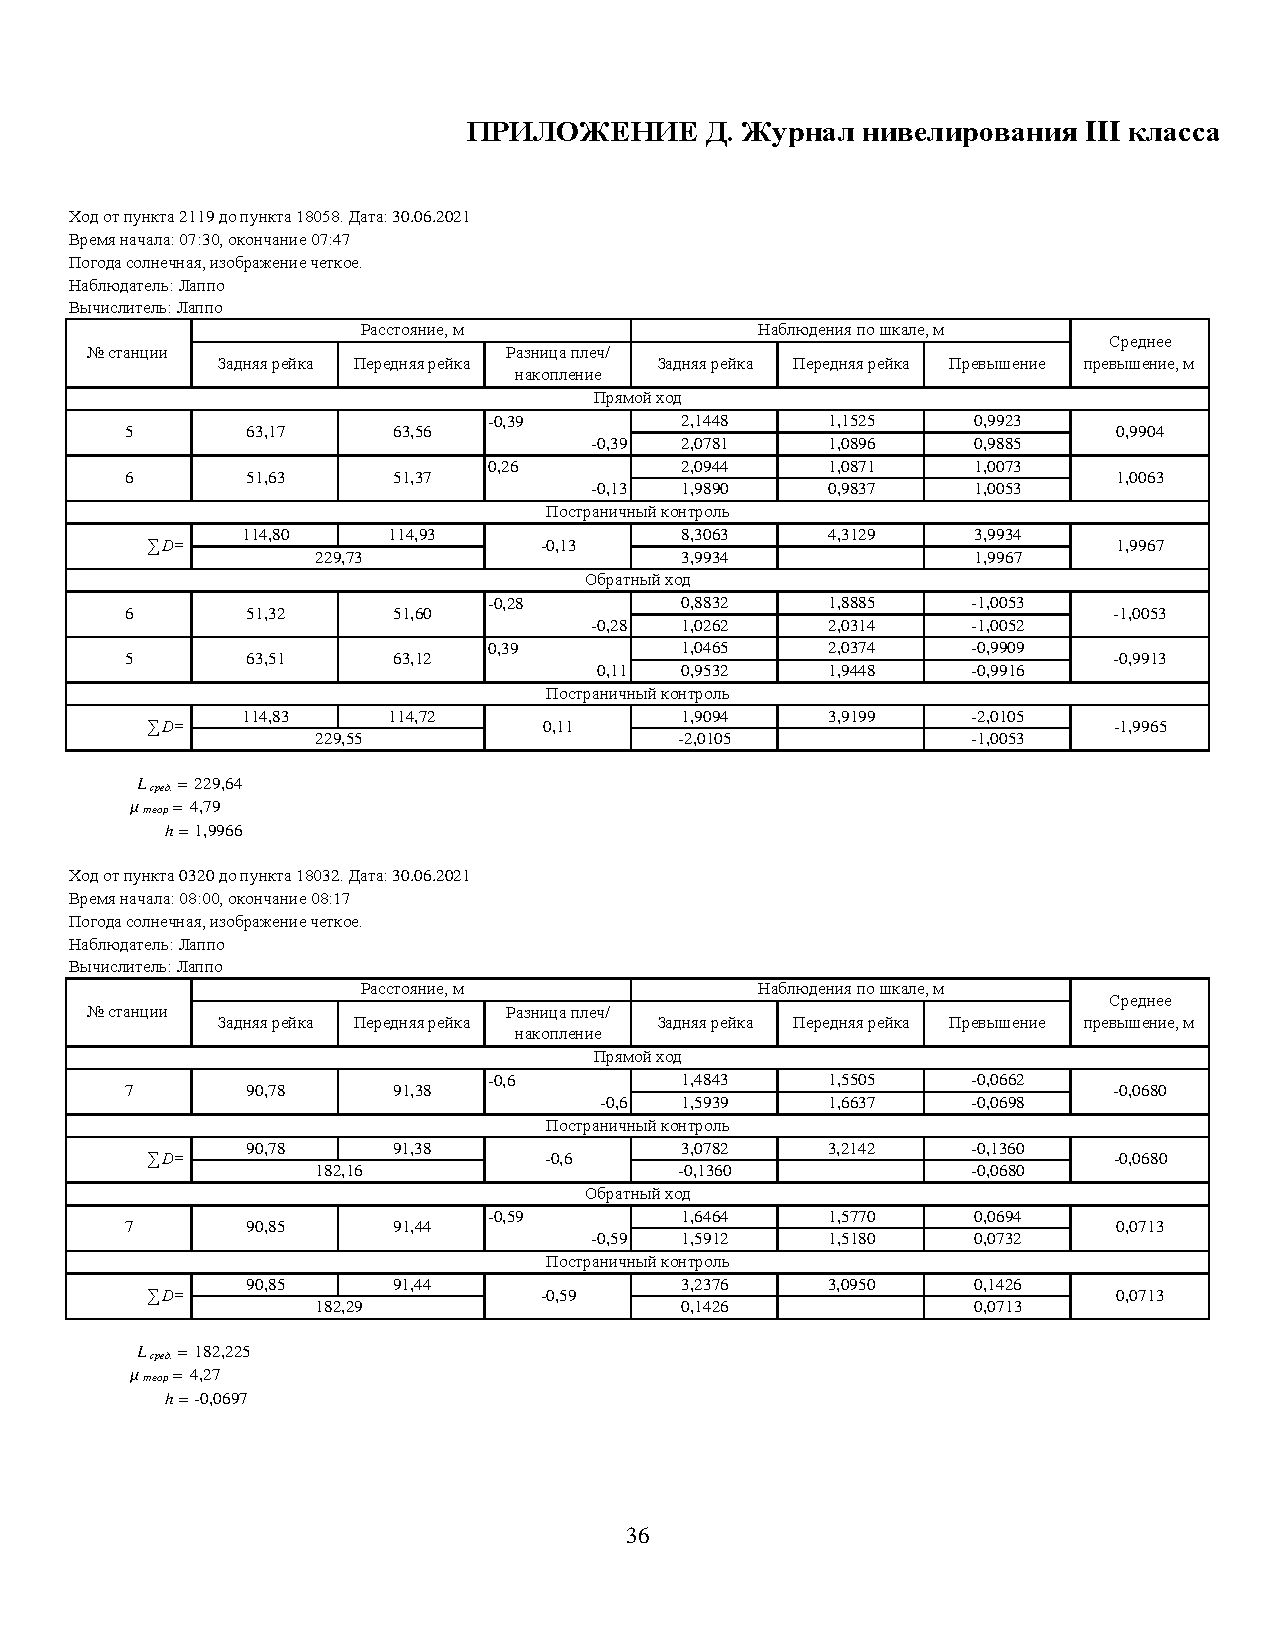
\includepdf[pages= - ]{5-21.pdf}
%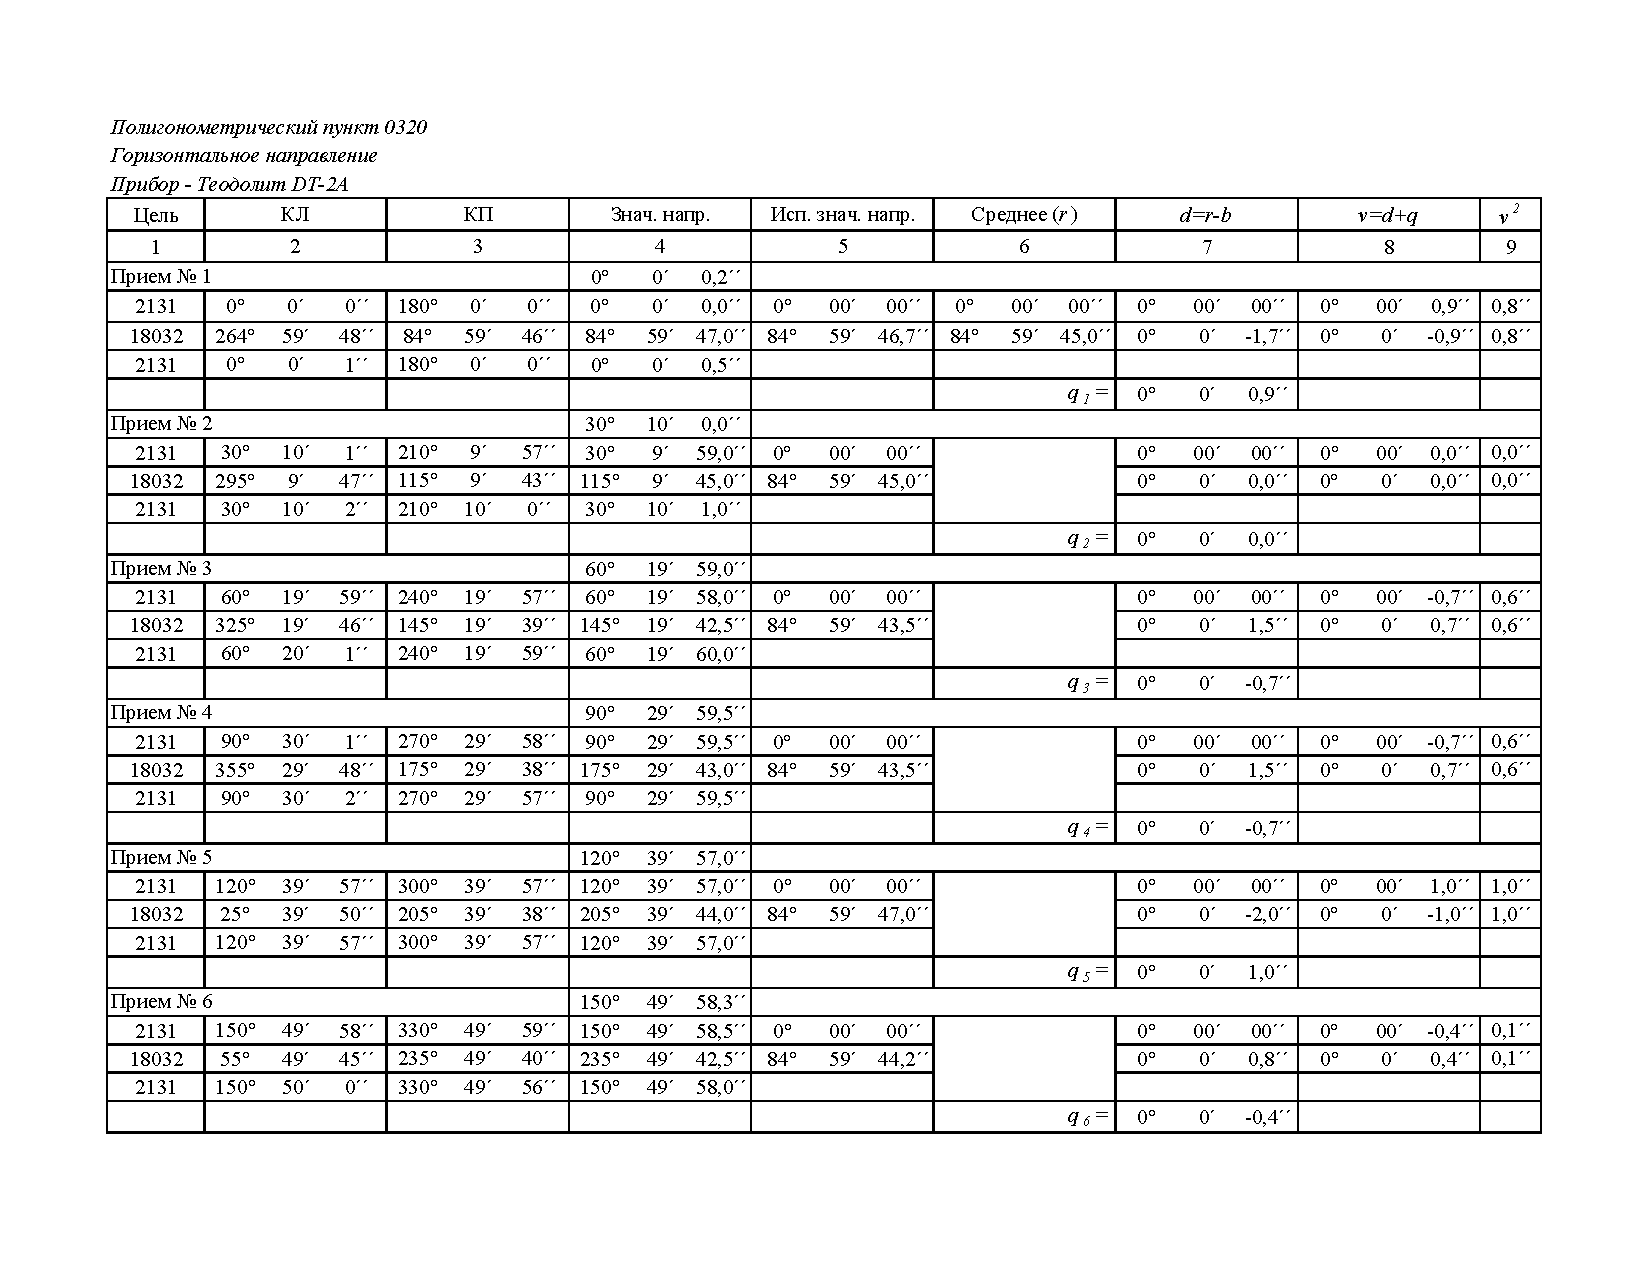
\includepdf[pages= - ]{Полигонометрия.pdf}
\begin{newpage}
\begin{flushright}
  \large{ПРИЛОЖЕНИЕ Е. Схема сети полигонометрии}
\end{flushright}
\begin{center}
    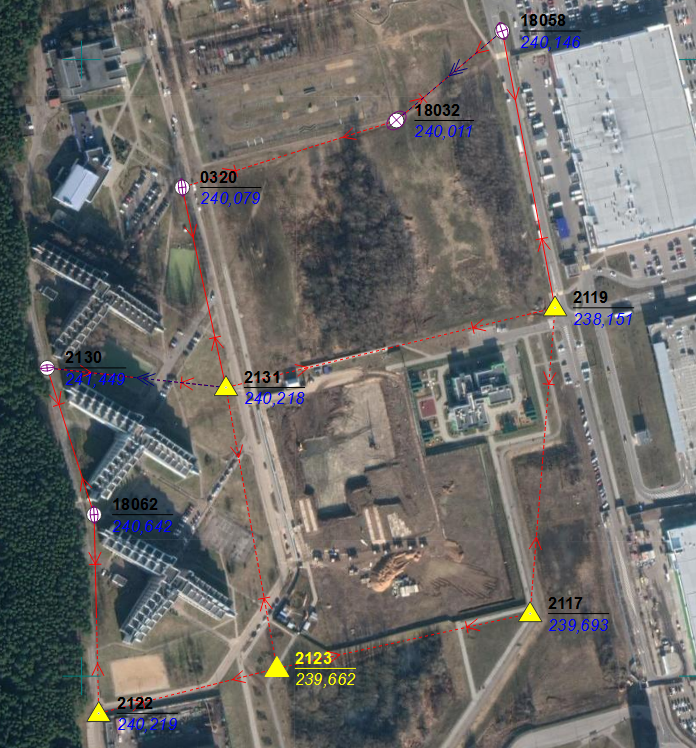
\includegraphics[scale=1]{1.png}
\end{center}
\end{newpage}
\end{newpage}
\begin{newpage}
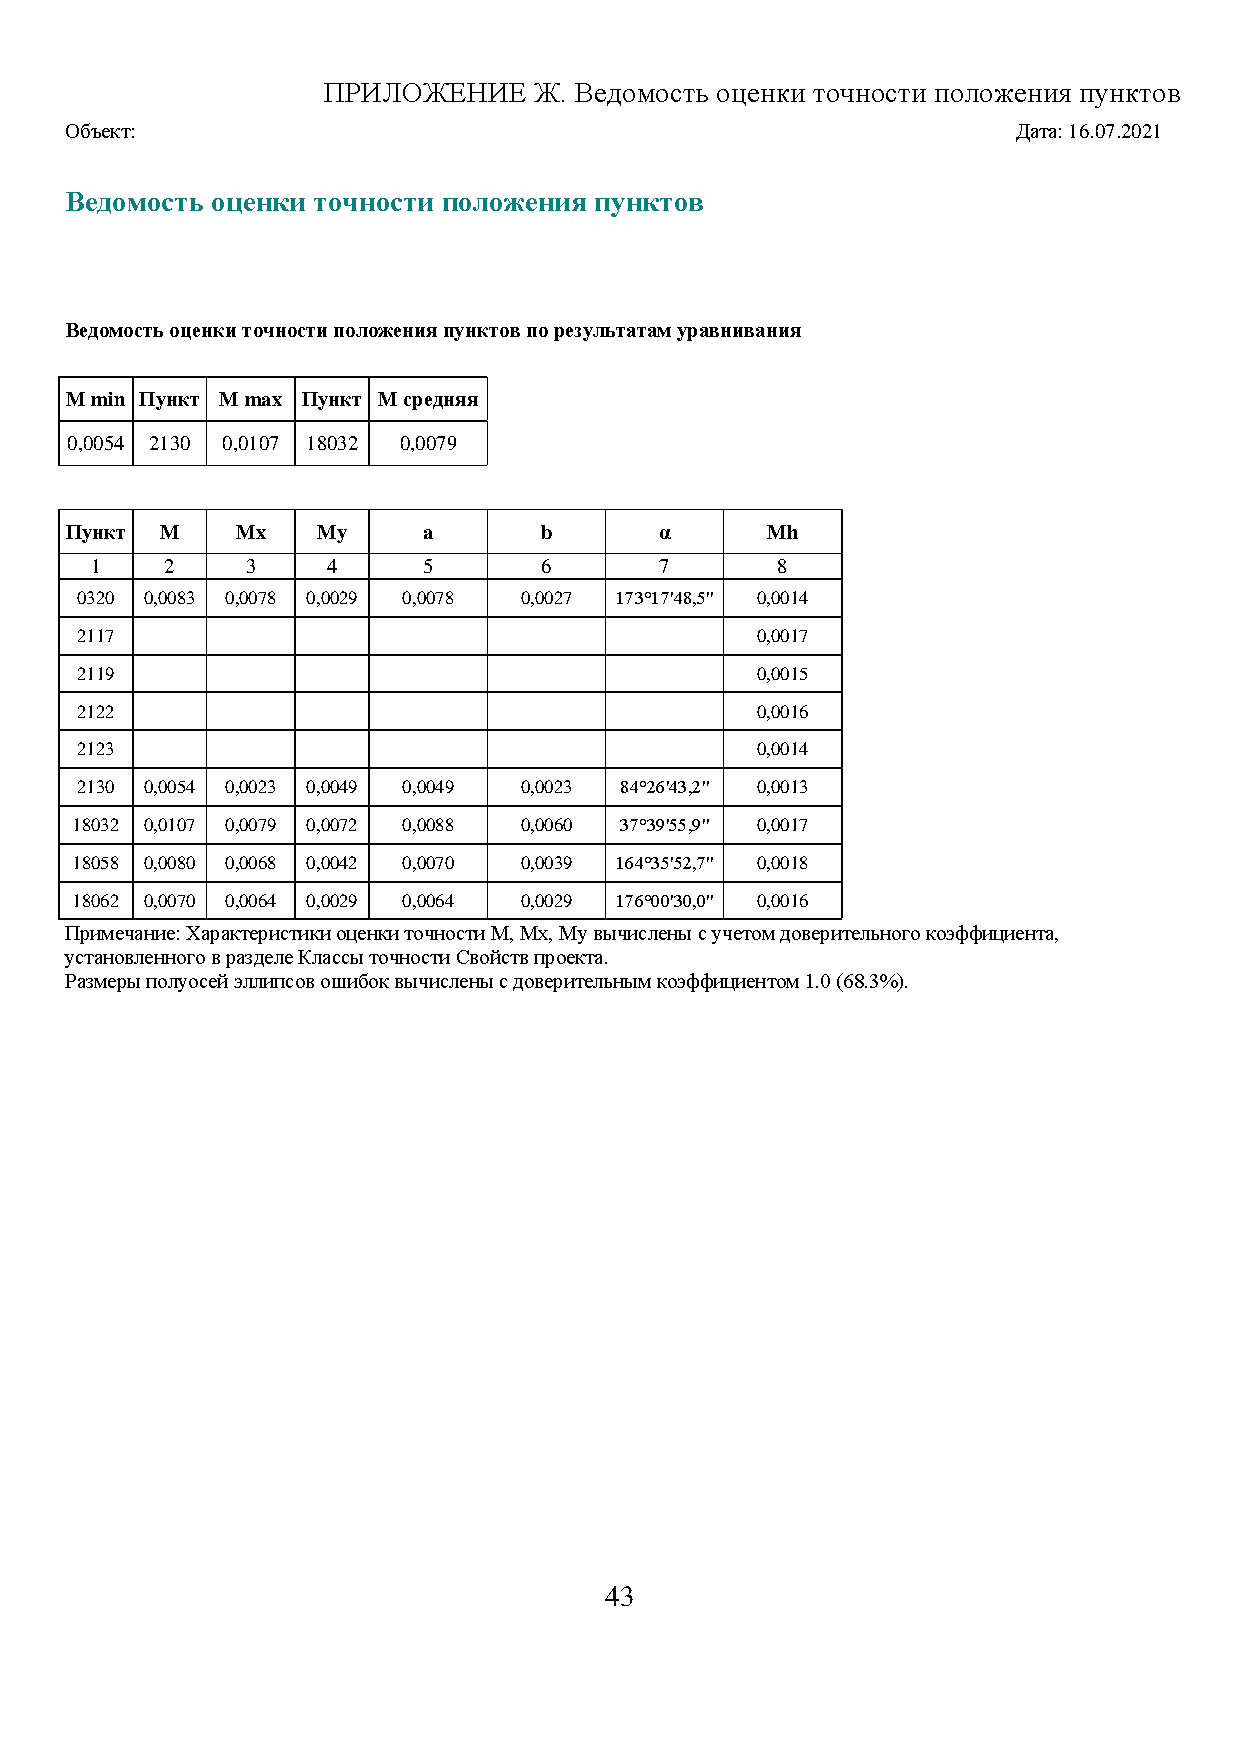
\includepdf[pages= - ]{2.pdf}
\end{newpage}

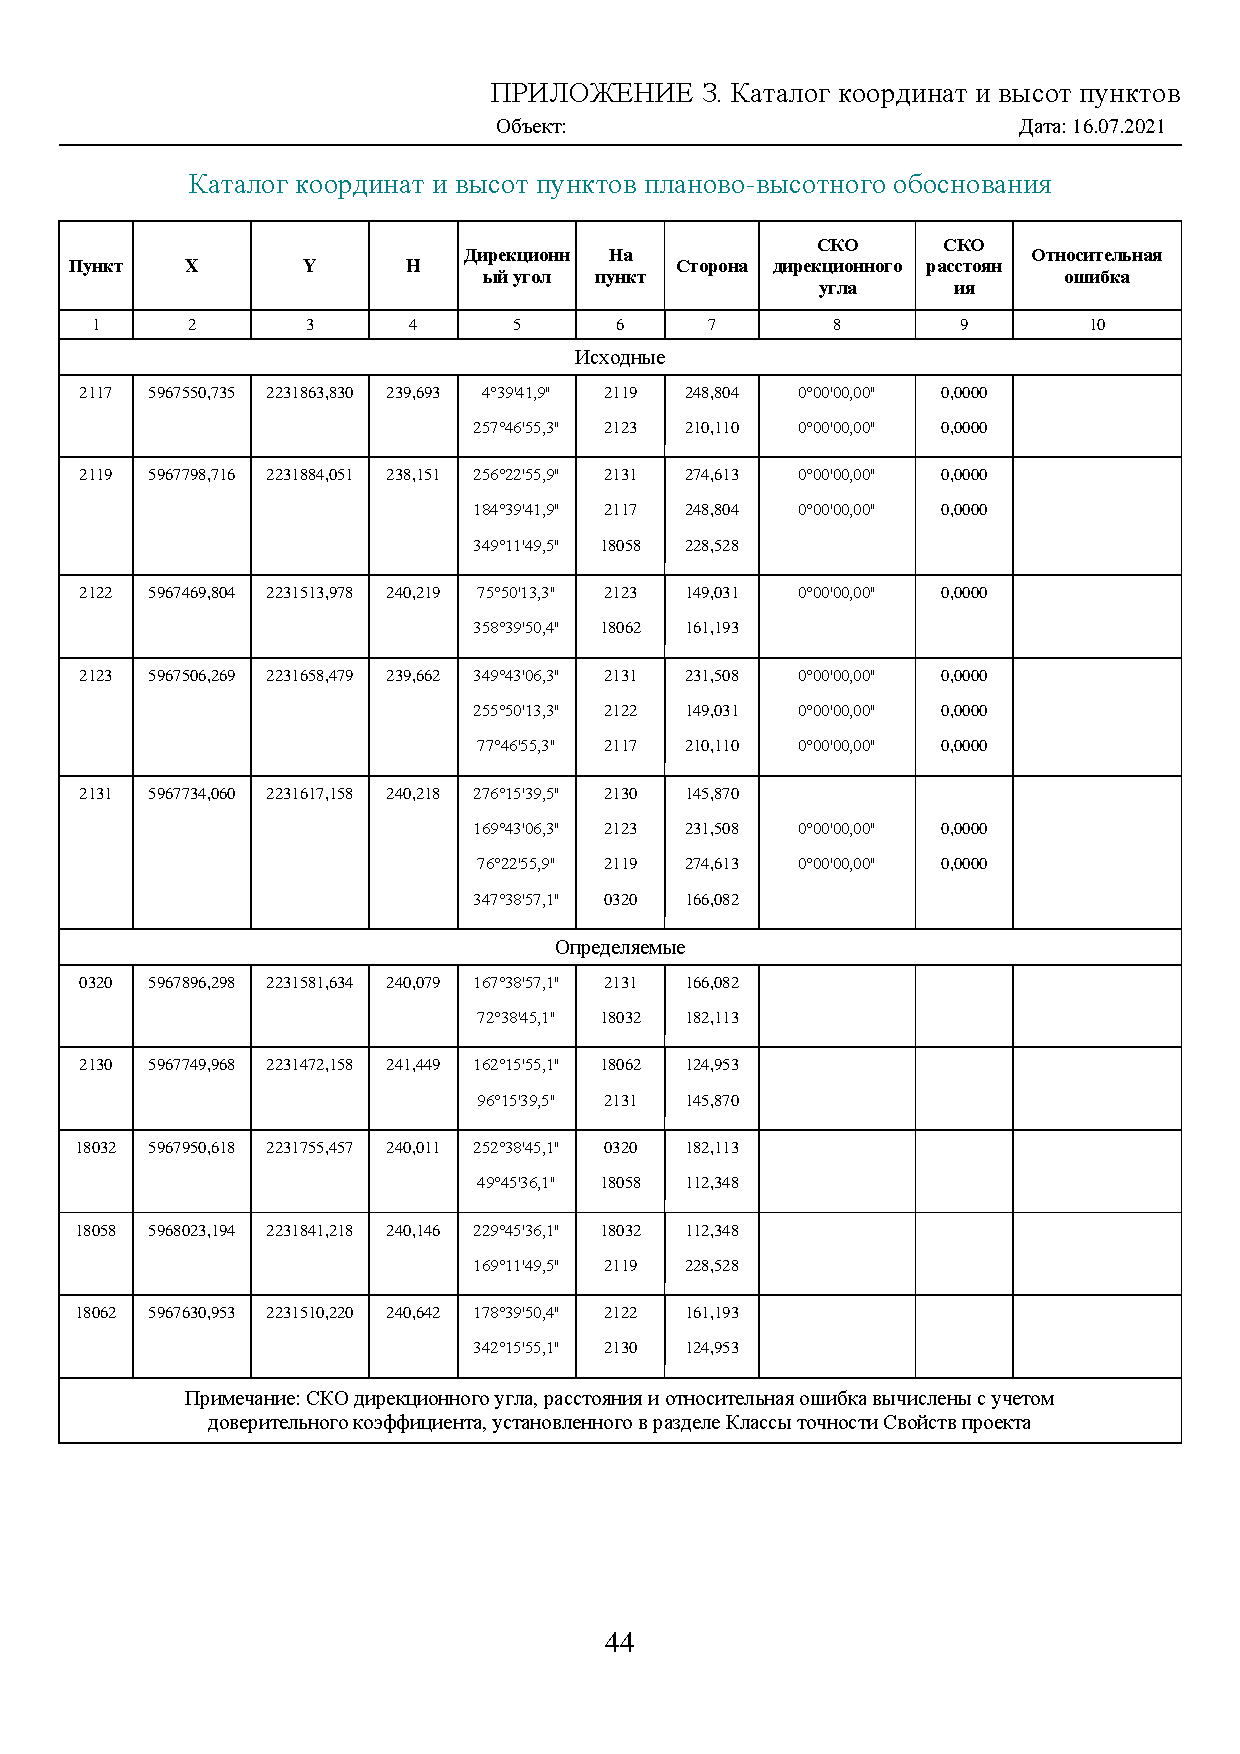
\includepdf[pages= - ]{3.pdf}
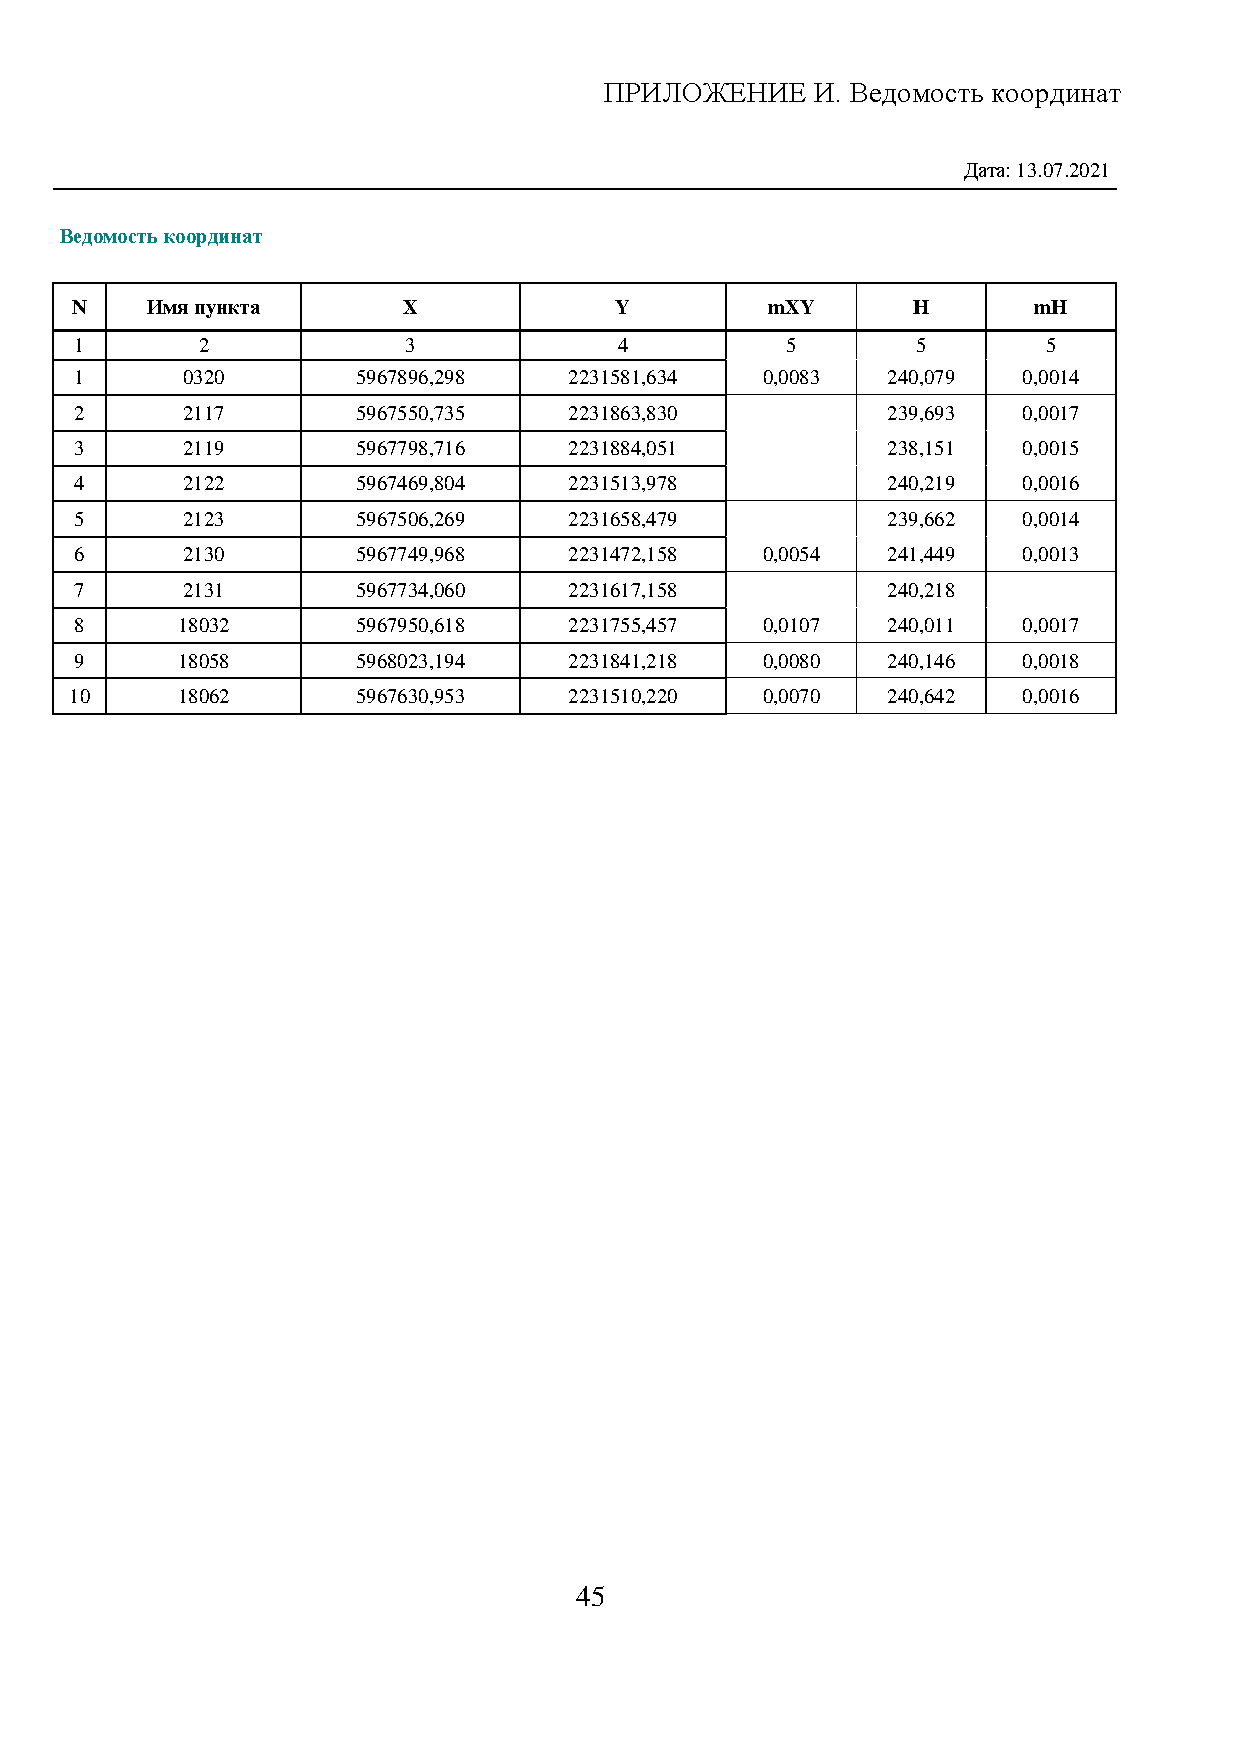
\includepdf[pages= - ]{4.pdf}
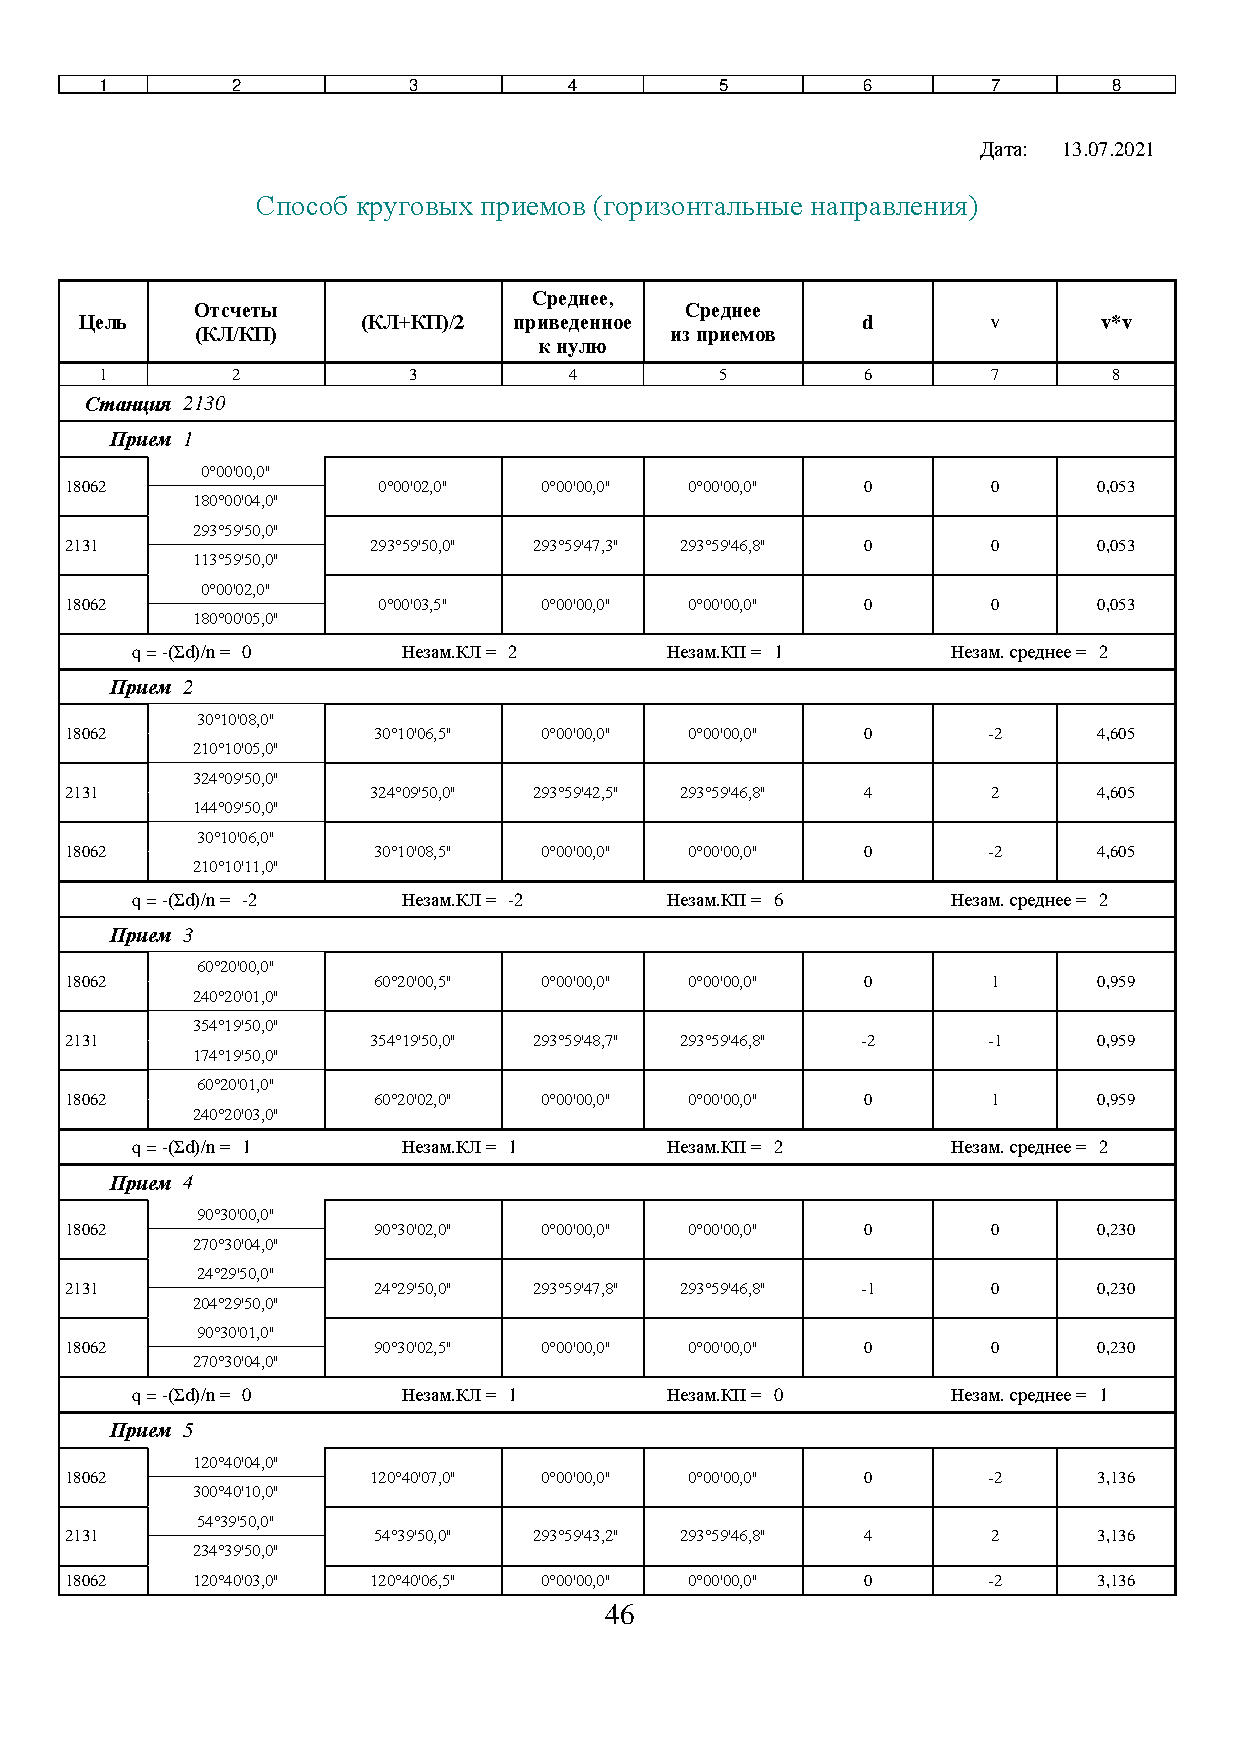
\includepdf[pages= - ]{5.pdf}
\end{document}